% !TeX document-id = {b5392a94-51a3-49d1-9ba5-698bc09f9d35}
% !TeX encoding = UTF-8
% !TeX spellcheck = en_US
% !TeX TXS-program:bibliography = biber -l zh__pinyin --output-safechars %

\documentclass[a4paper
	,10pt
%	,twoside
]{article}

% to be `\input` in subfolders,
% ... therefore the path should be relative to subfolders.

\usepackage{iftex}
\ifPDFTeX
\else
	\usepackage[UTF8
		,heading=false
		,scheme=plain % English Document
	]{ctex}
\fi
%\ctexset{autoindent=true}
\usepackage{indentfirst}

\input{../.modules/basics/macros.tex}
\input{../.modules/preamble_base.tex}
\input{../.modules/preamble_beamer.tex}
\input{../.modules/basics/biblatex.tex}


%Misc
	\usepackage{lilyglyphs}
	\newcommand{\indicator}{$\text{\clefG}$}
	\newcommand{\indicatorInline}{$\text{\clefGInline}$}

\newcommand{\legacyReference}{{
%	\clearpage\par
%	\quad\clearpage
	\def{\midquote}{\textbf{PAST WORK, AS TEMPLATE}}
	\newparagraph
}}

% Settings
\counterwithout{equation}{section}
\mathtoolsset{showonlyrefs=false}
%\DeclareTextFontCommand{\textbf}{\sffamily}

% Spacing
\geometry{footnotesep=2\baselineskip} % pre footnote split
\setlength{\parskip}{.5\baselineskip}
\renewcommand{\baselinestretch}{1.15}


%% List
%	\setlist*{
%		listparindent=\parindent
%		,labelindent=\parindent
%		,parsep=\parskip
%		,itemsep=1.2\parskip
%	}


\addtobeamertemplate{navigation symbols}{}{%
    \usebeamerfont{footline}%
%    \usebeamercolor[fg]{footline}%
    \hspace{1em}%
    \large\insertframenumber/\inserttotalframenumber
}

\makeatletter
\setbeamertemplate{headline}
{%
    \begin{beamercolorbox}[wd=\paperwidth,colsep=1.5pt]{upper separation line head}
    \end{beamercolorbox}
    \begin{beamercolorbox}[wd=\paperwidth,ht=2.5ex,dp=1.125ex,%
      leftskip=.3cm,rightskip=.3cm plus1fil]{title in head/foot}
      \usebeamerfont{title in head/foot}\insertshorttitle
    \end{beamercolorbox}
    \begin{beamercolorbox}[wd=\paperwidth,ht=2.5ex,dp=1.125ex,%
      leftskip=.3cm,rightskip=.3cm plus1fil]{section in head/foot}
      \usebeamerfont{section in head/foot}%
      \ifbeamer@tree@showhooks
        \setbox\beamer@tempbox=\hbox{\insertsectionhead}%
        \ifdim\wd\beamer@tempbox>1pt%
          \hskip2pt\raise1.9pt\hbox{\vrule width0.4pt height1.875ex\vrule width 5pt height0.4pt}%
          \hskip1pt%
        \fi%
      \else%  
        \hskip6pt%
      \fi%
      \insertsectionhead
    \end{beamercolorbox}
% Code for subsections removed here
}
\makeatother
\input{../.modules/basics/biblatex.tex}

\title{Notes on Gravitational Entropy}
\addbibresource{entropy.bib}

%%% ID: sensitive, do NOT publish!
\InputIfFileExists{id.tex}{}{}

\makeatletter
\newcommand{\nobeginpar}{\@beginparpenalty=10000}
\makeatother

\begin{document}
\maketitle
\pagenumbering{arabic}
\thispagestyle{empty}

%\vspace*{-.5\baselineskip}

\setlength{\parskip}{.1\baselineskip}
\tableofcontents
\setlength{\parskip}{\parskipnorm}

\addtocounter{section}{-1}
\section{Conventions}
	We try to follow the conventions of the TsT paper: \textcite{Apolo:2019zai}. 
	\begin{itemize}
	\item Lightcone coordinates: $u,v = x\pm t$, similar to \cite{Apolo:2019zai}. This convention has the following features:
	
		\begin{itemize}
		\item The constant $t$ slice is given by $u = v$;
		\item It preserves the orientation as we go from $(t,x)$ to $(u,v)$. Note that the ordering of coordinates matters here.
		\end{itemize}
	
	\item Poincar\'e $\mrm{AdS}_3$ coordinates: $
			X^I \sim (x^\mu,z) \sim (t,x,z) \sim (u,v,z)
		$, metric: $
			\dd{s}^2 = \frac{+\dd{u} \dd{v} + \dd{z}^2}{z^2}
		$. Note the \mquote{+} before $\dd{u} \dd{v}$. 
	
	\item The $T\bar{T}$ deformation is parametrized by the deformation parameter $\mu$, defined in \cite{Apolo:2019zai}; for the single-trace situation, it is more convenient to use the \textit{worldsheet} deformation parameter $\lambda = \mu/\ell_s^2$, where $\ell_s$ is the string length. See \cite{Apolo:2019zai} section 2.3 and its (2.43). 
	\end{itemize}
	
\pagebreak[4]
\section{Entanglement Entropy as Thermal Entropy}
	Ref: \textcite{Apolo:2020qjm}.
	
	A boundary interval $\mcal{A} \Leftrightarrow \rho_\mcal{A} = e^{-\mcal{H}_\mcal{A}}$. $\mcal{H}_\mcal{A}$ is generically nonlocal, but in a highly symmetric background (e.g.~vacuum) it might be geometrically realized and corresponds to a symmetry of the underlying quantum field theory.
	In this case there is a generalized Rindler transformation $f$ that maps the casual $\mcal{D} \to \{(\tau,\tilde{x})\}$ in some noncompact generalized Rindler spacetime, with $\pdd{\tau}$ an isometry of the spacetime. Then we have:
	\begin{equation}
		\xi = 2\pi \pdd{\tau}
		= 2\pi \sum_i a^i H_i,
	\quad
		\tau \sim \tau + 2\pi i
	\end{equation}
	$H_i$: symmetry generators. The causal domain of dependence $\mcal{D}\to$ some thermal state with normalized inverse temperature $2\pi$. Here we choose to absorb such $2\pi$ into the definition of $\xi$, so the Euclidean periodicity w.r.t.~$\xi$ is simply $\beta_\xi = 1 = \frac{1}{T_\xi}$, which means the surface gravity along the horizon is given by $\kappa_\xi = 2\pi T_\xi = 2\pi$. 
\subsection{Case study: Poincar\'e $\mrm{AdS}_3/\mrm{CFT}_2$}
	We illustrate the above ideas in Poincar\'e $\mrm{AdS}_3$ vacuum, which is the simplest situation and can be easily compared with the results of \textcite{Lewkowycz:2019xse}. 
\subsubsection{Bulk / boundary Killings}
	In Poincar\'e $\mrm{AdS}_3/\mrm{CFT}_2$, the $H_i$'s are given by $L_n,\bar{L}_n$ with $n=0,\pm 1$. At $z\to 0$ we recover the usual global $\mfrak{sl}(2,\mbb{R})$ generators:
	\begin{equation}
		z\to 0,
	\quad
		      L_n \to -u^{n+1} \pdd{u},\quad
		\bar{L}_n \to -v^{n+1} \pdd{v},\quad
	n = 0,\pm 1
	\end{equation}
	Q: Why we only include the global generators on the field theory side? A: These are the symmetries of the Poincar\'e vacuum. 
	
	One could argue that $L_{n>1}$ still annihilates the vacuum $\ket{0}$, however we should actually consider all possible correlations w.r.t.~$\ket{0}$, and require that they remain unchanged under variation of $\ket{0}$. This means that:
	\begin{equation}
		0 = \bqty{\rho,L_n}
		= \bqty\Big{\dyad{0},L_n}
	\end{equation}
	Note that $L^\dagger_n = L_{-n}$, we thus have the restriction that $n = 0,\pm 1$. 
	
	To extend it to the bulk, think of the corresponding bulk isometries: translations, rotations, dilations and special conformal transformations:
	\begin{equation}
	\begin{aligned}
		P_\mu
		&= \pdd{\mu},\\
		m_{uv}
		&= x_\mu \pdd{\nu} - x_\nu \pdd{\mu}
		= u\pdd{u} - v\pdd{v},\\
		\Delta
		&= X^I \pdd{I}
		= u\pdd{u} + v\pdd{v} + z\pdd{z},\\
		K_\mu
		&= (z^2 + uv)\,\pdd{\mu}
			- 2\eta_{\mu\nu} x^\nu \Delta,
	\end{aligned}
	\end{equation}
	\begin{equation}
		K_u = (z^2 + uv)\,\pdd{u} - v \Delta,
	\quad
		K_v = (z^2 + uv)\,\pdd{v} - u \Delta
	\end{equation}
	By requiring that a linear combination of these generators reduce to the boundary $L_n$'s, one can uniquely extend the $L_n,\bar{L}_n$'s into the bulk; see \texttt{modFlowPoincare.nb}. The result for $L_n$'s is listed below; for $\bar{L}_n$ one need only exchange all $u\leftrightarrow v$.
	\begin{equation}
		L_{-1} = -\pdd{u},
	\quad
		L_0 = -u\,\pdd{u} - \frac{z}{2}\,\pdd{z},
	\quad
		L_1 = -u^2\pdd{u} + z^2 \pdd{v}
			- uz\,\pdd{z}
	\end{equation}
\subsubsection{Bulk modular flow}
	The RT surface (spacelike geodesic of Poincar\'e AdS with both ends attached to the boundary) is parametrized in terms of its end points $(t,x)_\pm$; it's the intersection of a ``sphere'' (hyperboloid) and a plane through its center:
	\begin{equation}
	\text{``sphere'':}\quad
		z^2
		+ \pqty{x - \frac{x_+ + x_-}{2}}^{\!\!2}
		- \pqty{t - \frac{t_+ + t_-}{2}}^{\!\!2}
		= \pqty{\frac{L}{2}}^{\!\!2}
		= \pqty{\frac{x_+ - x_-}{2}}^{\!\!2}
		- \pqty{\frac{t_+ - t_-}{2}}^{\!\!2}
	\end{equation}
	\begin{equation}
		L^2
		= \pqty{x_+ - x_-}^2
			- \pqty{t_+ - t_-}^2
		= (u_+ - u_-)(v_+ - v_-)
	\end{equation}
	\begin{equation}
	\text{plane:}\quad
		\frac{x - \frac{1}{2} (x_+ + x_-)}{x_+ - x_-}
		= \frac{t - \frac{1}{2} (t_+ + t_-)}{t_+ - t_-}
	\end{equation}
	See \href{https://bryango.github.io/resources/archive/HW-Gravity/gravity1.pdf}{\textsl{this homework}}\footnote{
		URL: \https{bryango.github.io/resources/archive/HW-Gravity/gravity1.pdf}. 
	} for a detailed derivation. 
	Alternatively, it can be more compactly rewritten with $x^\mu \sim (t,x)$ or $(u,v)$; mind the various $\pm$ signs in the above expressions: 
	\begin{equation}
	\begin{aligned}
		0 &= z^2
			+ \eta_{\mu\nu} (x - x_+)^\mu (x - x_-)^\nu \\
		& = z^2
			+ (x - x_+)(x - x_-)
			- (t - t_+)(t - t_-) \\
		&= z^2 + \frac{
				(u - u_+)(v - v_-)
				+ (v - v_+)(u - u_-)
			}{2}
	\end{aligned}
	\end{equation}
	
	The bulk modular generator vanishes along the RT surface, i.e.~the RT surface is the fixed point of the modular flow; with this condition we can fix the coefficients of the modular generator, up to an overall coefficient\footnote{
		One can compare this with similar results in the literature such as \cite{Lashkari:2016idm,Czech:2019vih,Apolo:2020qjm}. 
	}:
	\begin{equation}
		\xi = 2\pi \sum_{n=0,\pm 1} \pqty{
				s_n L_n - \bar{s}_n \bar{L}_n
			},
	\end{equation}
	\begin{equation}
		s_{-1} = \frac{u_+ u_-}{u_+ - u_-},\quad
		s_0 = - \frac{u_+ + u_-}{u_+ - u_-},\quad
		s_{+1} = \frac{1}{u_+ - u_-}
	\end{equation}
	One need only exchange all $u\leftrightarrow v$ to obtain $\bar{s}_n$. The overall coefficient of $\xi$ (in this case, $2\pi$) is fixed by normalizing the temperature of the horizon, namely we demand that the surface gravity is $2\pi$ along the RT surface:
	\begin{equation}
		T_\xi = \frac{\kappa_\xi}{2\pi} = 1,
	\quad
		\kappa_\xi^2
		= (2\pi)^2
		= -\frac{1}{2}\,
			(\nabla_{\mu} \xi_{\nu})
			(\nabla^{\mu} \xi^{\nu})
	\end{equation}
	
\subsubsection{Modular flow at the cutoff surface}
	We now restrict to an interval centered at the origin: $
		u_\pm v_\pm
		= x^2_\pm - t^2_\pm
		= (\frac{L_\infty}{2})^2
	$, $x_\pm = -x_\mp$, and same for $t_\pm, u_\pm, v_\pm$. 
	We then introduce the \textit{rapidity} variable $\theta$ to nicely parametrized the boosted interval; for a constant time slice, we have $\theta = 0$. For a general boosted interval, we have:
	\begin{equation}
		x_\pm = \pm \frac{L_\infty}{2} \cosh \theta,
	\quad
		t_\pm = \pm \frac{L_\infty}{2} \sinh \theta,
	\end{equation}
	For now the coordinates $u_\pm, v_\pm, x_\pm, t_\pm$ and the coordinate length $L_\infty$ are all specified at $z\to 0$, i.e.~at the \textbf{asymptotic boundary}. Note that the RT surface lies on the plane $
		t_\pm / x_\pm = \tanh \theta
	$, namely $\theta$ is constant along the RT surface. 
	We have:
	\begin{gather}
	\begin{aligned}
		\xi &= \frac{2\pi}{L_\infty} \bigg\{
			\pqty\Big{
				\pqty{
					(\tfrac{L_\infty}{2})^2 - z^2
					- (t^2 + x^2)
				} \cosh\theta
				+ 2tx \sinh\theta
			} \,\pdd{t}
		\\ &\qquad\qquad 
			+ \pqty\Big{
				\pqty{
					(\tfrac{L_\infty}{2})^2 - z^2
					+ (t^2 + x^2)
				} \sinh\theta
				- 2tx \cosh\theta
			} \,\pdd{x}
		\\ &\qquad\qquad 
			+ \pqty\big{
				x\sinh\theta
				- t\cosh\theta
			} \,2z\pdd{z}
		\bigg\}
	\end{aligned}
	\end{gather}
	
\pagebreak[3]
	We see that the $\pdd{z}$ term vanishes in the following two cases:
	\begin{itemize}[noitemsep]
	\item as $z\to 0$, i.e.~near the asymptotic boundary;
	\item within the whole plane $
			x\sinh\theta
			= t\cosh\theta
		$ where the RT surface lies. 
	\end{itemize}
	Now we'd like to study $\xi$ not at the asymptotic boundary, but at some \textbf{constant finite cutoff} $z = z_c$. 
	Note that is the size (coordinate length) of the interval at the {asymptotic boundary}; the coordinate length of the \textbf{cutoff interval $L$}, on the other hand, is given by:
	\begin{equation}
		\pqty{\frac{L}{2}}^{\!\!2}
		= \pqty{\frac{L_\infty}{2}}^{\!\!2} - z_c^2,
	\quad
		x_\pm^c
		= \pm \frac{L}{2}
	\label{eq:length_relations}
	\end{equation}
	
	We then consider $\xi$ evaluated at the {constant finite cutoff} $z = z_c$,
	\begin{equation}
	\begin{aligned}
		\xi|_{z=z_c}
		= \frac{2\pi}{
				L\sqrt{1 + (2z_c/L)^2}
			}
		& \bigg\{
			\pqty\Big{
				\pqty{
					(\tfrac{L}{2})^2
					- (t^2 + x^2)
				} \cosh\theta
				+ 2tx \sinh\theta
			} \,\pdd{t}
		\\[-.5ex] &\quad 
			+ \pqty\Big{
				\pqty{
					(\tfrac{L}{2})^2
					+ (t^2 + x^2)
				} \sinh\theta
				- 2tx \cosh\theta
			} \,\pdd{x}
		\\ &\quad 
			+ \pqty\big{
				x\sinh\theta
				- t\cosh\theta
			} \,2z_c\pdd{z}
		\bigg\}
	\end{aligned}
	\end{equation}
	Note that the $\pdd{z}$ component is generally non-zero, i.e.~$\xi|_{z=z_c}$ is not entirely contained in the $z = z_c$ plane. 
	We observe the factor $
		\sqrt{1 + (2z_c/L)^2}
	$ which is featured prominently in the $T\bar{T}$ deformed $C(L)$ function, given in \cite{Lewkowycz:2019xse}:
	\begin{equation}
		C(L) = L\,\pdd{L} S(L)
		= \frac{c}{3} 
			\frac{1}{
				\sqrt{1 + (2z_c/L)^2}
			}
	\end{equation}
	
	This seems nice and all but there is a subtlety for finite cutoff $z = z_c$. 
	In the bulk the constant surface gravity $
		\xi^\nu \cdv{\nu} \xi^\mu
		= \kappa_\xi \xi^\mu
		= 2\pi \xi^\mu
	$ guarantees that after Wick rotation, the Euclidean periodicity around the horizon is normalized to $\beta = 1$. However, if we restrict to the field theory living at $z = z_c$, which corresponds to a $T\bar{T}$ deformed theory, since it has no knowledge of the $\pdd{z}$ component of $\xi$, we should reduce it to a modular flow within the $z = z_c$ plane by, e.g.~projecting the $z$ component out, which leaves us:
	\begin{equation}
	\begin{aligned}
		\xi^{\mrm{FT}}_c
		\equiv \proj{\sslash} \xi|_{z_c}
		= \frac{2\pi}{
				\sqrt{1 + (2z_c/L)^2}
			}
		& \bigg\{
			\pqty\Big{
				\pqty{
					(\tfrac{L}{2})^2
					- (t^2 + x^2)
				} \cosh\theta
				+ 2tx \sinh\theta
			} \,\pdd{t}
		\\[-2ex] &\quad 
			+ \pqty\Big{
				\pqty{
					(\tfrac{L}{2})^2
					+ (t^2 + x^2)
				} \sinh\theta
				- 2tx \cosh\theta
			} \,\pdd{x}
		\bigg\}
	\end{aligned}
	\end{equation}
	Which no longer has normalized $\beta$ if $z_c \ne 0$. In fact, compared to the $z_c \to 0$ situation which \textit{does} have $\beta = 1$, $\xi^{\mrm{FT}}_c$ is rescaled by a factor of $
		\frac{L}{L_\infty}
		= 1/\sqrt{1 + (2z_c/L)^2}
	$, which means that:
	\begin{equation}
		\beta^{\mrm{FT}}_c
		= \sqrt{1 + (2z_c/L)^2}
		\sim 1 + 2z_c^2 / L^2
	\end{equation}
	
{\nobeginpar
	How should we understand this?
	\begin{itemize}
	\item The $T\bar{T}$ deformation might somehow correspond to a variation of temperature at the cutoff; instead of $\rho = e^{-\mcal{H}}$, we now have:
	\begin{equation}
		\rho = e^{-\beta\mcal{H}},
	\quad \beta \sim 1 + \frac{1}{L^2} \order{\mu}
	\end{equation}
	Where $\mu$ is the deformation parameter (see \cite{Apolo:2019zai} for the convention we follow). Q: how do we make this precise?
	
	\item The non-local nature of $T\bar{T}$ deformation creates some $\order{z_c}$ ``fuzziness'' in the cutoff theory at $z = z_c$; $\beta \sim 1$ holds, but only up to some coarse-graining of points. Q: again, how do we make this precise?
	
	\item Instead of projecting out the $\pdd{z}$ component of $\xi$, maybe we could \textit{define} the evolution of the cutoff interval by following the flow of $\xi = 2\pi\pdd{\tau}$ starting from the RT surface at $z = z_c$. Now there is no longer a projection of $\xi$; we are always following it along the boundary, so the periodicity is preserved: $\beta = 1$. 
	
	But now this is no longer a \textit{constant} cutoff away from $z = z_c$. In particular, the forward and backward evolved interval will approach the upper and lower endpoints of the diamond at $z \to 0$. Q: does this make sense? Will it be compatible with \textcite{McGough:2016lol}?
	\end{itemize}
}
	
	\begin{figure}[!ht]
	\vspace{-1.5ex}
	\centering
	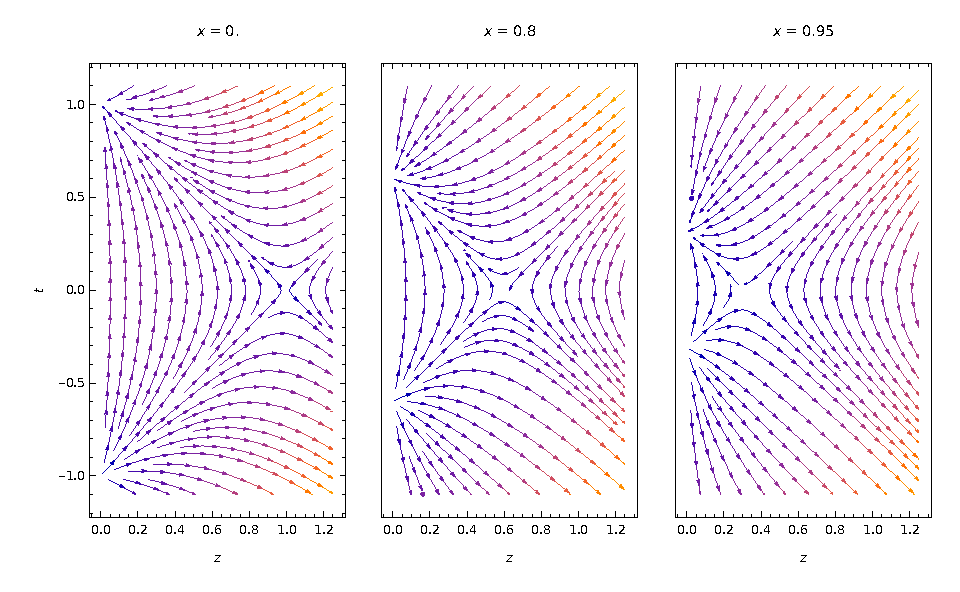
\includegraphics[width=.8\linewidth]{img/modFlowXsection.pdf}
	\hspace{2em}
	\vspace{-2ex}
	\caption{Modular flow at constant $x$ slices}
	\end{figure}
	
	\begin{figure}[!ht]
	\centering
%	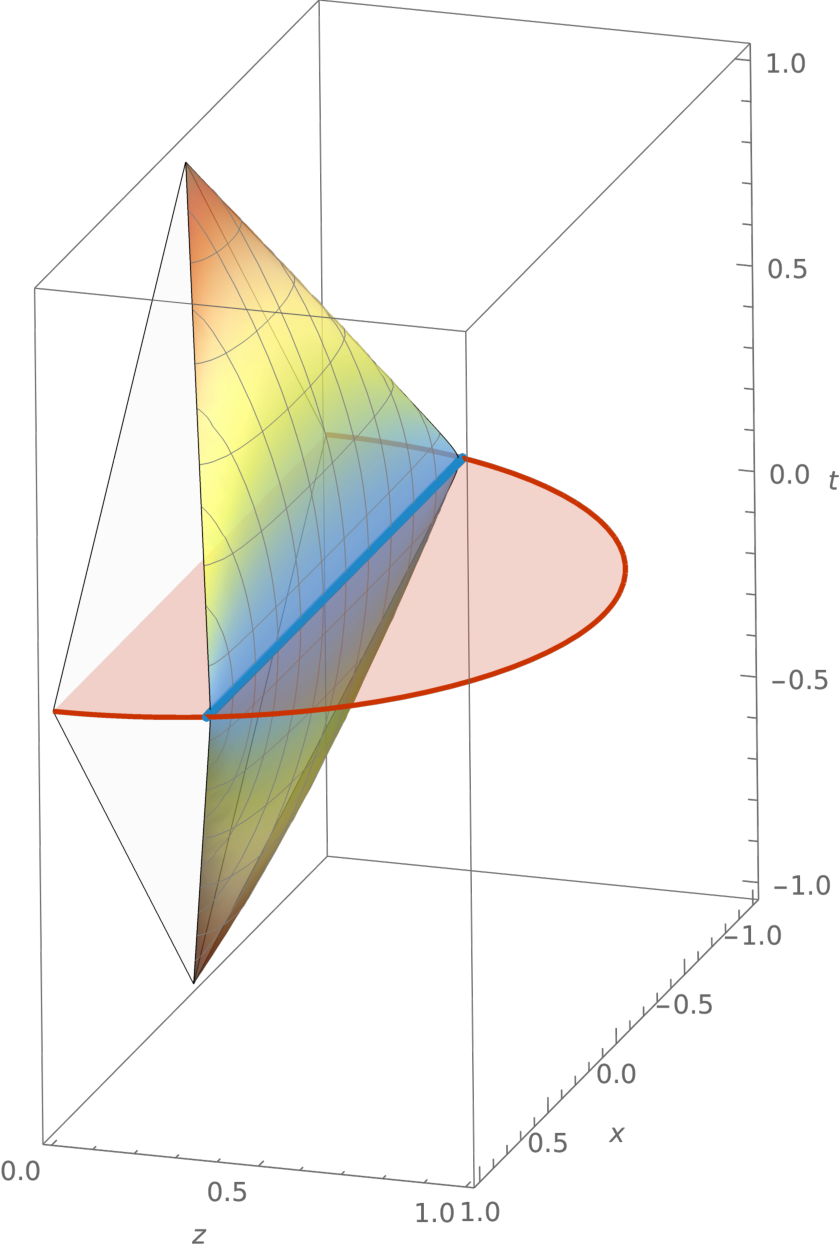
\includegraphics[width=.35\linewidth]{img/modFlowCutoff.pdf}
	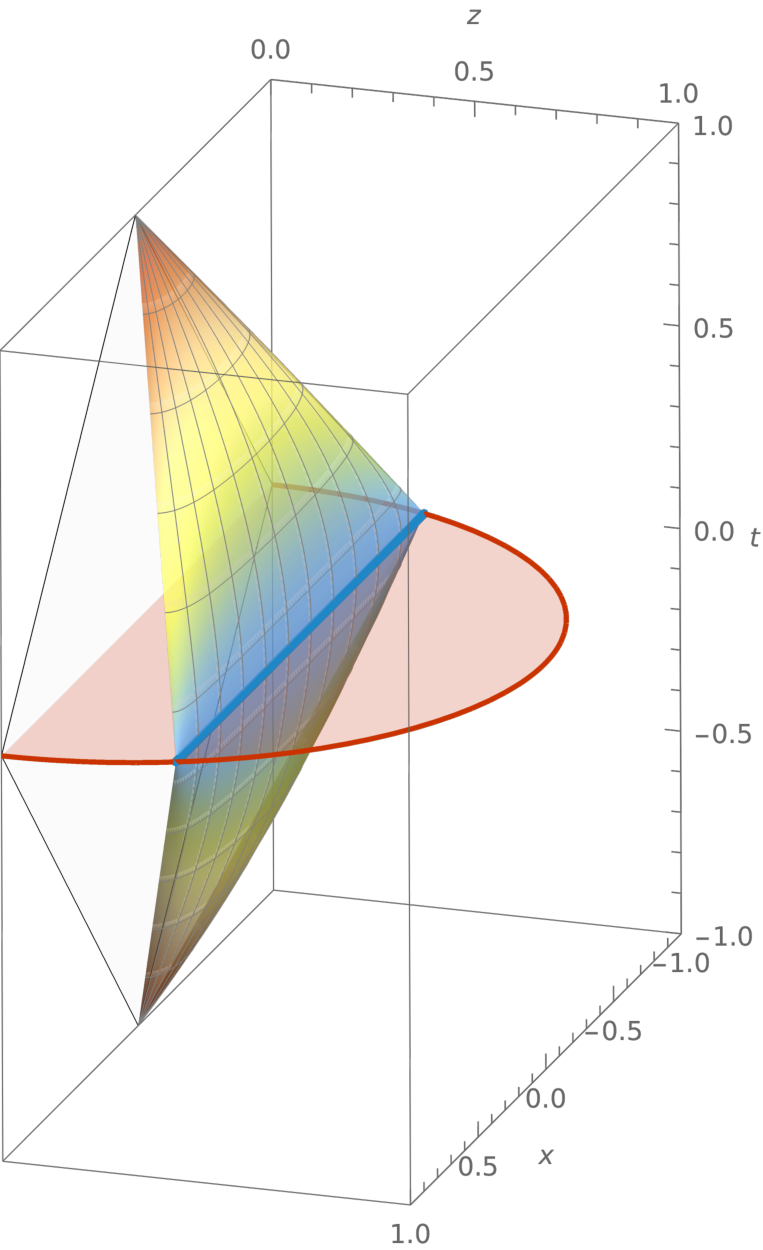
\includegraphics[width=.35\linewidth]{img/modFlowAnalytic.pdf}
%	\hspace{2em}
%	\vspace{-2ex}
	\caption{Integral surface of the modular flow starting from $t = 0,\ z = z_c$. Here we've chosen $\frac{L_\infty}{2} = 1$ while $z_c = 0.4$.}
	\end{figure}
	
\subsubsection{Flow from constant cutoff}
	For an interval lying on a constant time slice $t_\pm = 0$, i.e.~$\theta = 0$, we can actually solve the flow of $\xi$ by hand without much difficulty.
	
	Consider the flow starting from $(t,x,z) = (0,x_c,z_c)$, we note that $
		\dd{x}/\dd{z}
		= {\dv{x}{\lambda}}/{\dv{z}{\lambda}}
		= {x}/{z}
	$, which implies that ${x}/{x_c} = {z}/{z_c}$ along the flow lines. Intuitively, the flow when restricted in $x$-$z$ plane points towards / away froms $x = z = 0$, which is the upper / lower tip of the entanglement wedge. 
	
	We can further replace the flow parameter $\lambda$ with time coordinate $t$ by considering $
		\dd{z}/\dd{t}
		= {\dv{z}{\lambda}}/{\dv{t}{\lambda}}
	$, which leads to the following equations:
	\begin{equation}
		\dv{z}{t}
		= \frac{2tz}{\alpha z^2 + t^2 - (L_\infty/2)^2},
	\quad
		\alpha = 1 + \frac{x_c^2}{z_c^2},
	\quad
		\frac{x}{x_c} = \frac{z}{z_c}
	\end{equation}
	The solution is then given by:
	\begin{equation}
		z = z(t;x_c,z_c)
		= \frac{
				(L_\infty/2)^2 + \alpha z_c^2
				- \sqrt{
					\pqty\big{(L_\infty/2)^2 - \alpha z_c^2}^2
					+ 4t^2 \alpha z_c^2
				}
			}{2\alpha z_c}
	\end{equation}
	
	
	
%\subsubsection{Map to the Rindler coordinates}
	To gain more understanding of the modular flow of the cutoff theory, we can look at the map to the Rindler coordinates. In the Poincar\'e $\mrm{AdS}_3$ case this is explicitly given in Appendix B by \textcite{Song:2016gtd}; the entanglement wedge in Poincar\'e $(t,x,z)$ is mapped to the planar BTZ $(u,v,\rho)$:
	\begin{equation}
	\begin{aligned}
		t &= \frac{L_\infty}{2} \frac{
				\pqty{\rho - T_u T_v}
				\,\sinh\,(T_u u - T_v v)
			}{
				\sqrt{\rho^2 - T_u^2 T_v^2}
					\,\cosh\,(T_u u + T_v v)
				+ \pqty{\rho - T_u T_v}
					\,\cosh\,(T_u u - T_v v)
			},
	\\
		x &= \frac{L_\infty}{2} \frac{
				\sqrt{\rho^2 - T_u^2 T_v^2}
				\,\sinh\,(T_u u + T_v v)
			}{
				\sqrt{\rho^2 - T_u^2 T_v^2}
					\,\cosh\,(T_u u + T_v v)
				+ \pqty{\rho - T_u T_v}
					\,\cosh\,(T_u u - T_v v)
			},
	\\
		z &= \frac{L_\infty}{2} \frac{
				\sqrt{2T_u T_v}
				\sqrt{\rho - T_u T_v}
			}{
				\sqrt{\rho^2 - T_u^2 T_v^2}
					\,\cosh\,(T_u u + T_v v)
				+ \pqty{\rho - T_u T_v}
					\,\cosh\,(T_u u - T_v v)
			},
	\end{aligned}
	\label{eq:poincare2btz}
	\end{equation}
	\begin{equation}
		\dd{s}^2
		= \frac{\dd{\rho}^2}{4\,(\rho^2 - T_u^2 T_v^2)}
			+ T_u^2 \dd{u}^2
			+ T_v^2 \dd{v}^2
			+ 2\rho \dd{u} \dd{v},
	\end{equation}
	This is a BTZ \textit{black string} with \textit{non-compact} $\phi$ direction. 
	One can check that the $(u,v,\rho)$ coordinates indeed cover the $L_\infty$-sized entanglement wedge specified by $\xi$. 
	Here we've reused the variable names $(u,v)$ for the planar BTZ coordinates, and we've tweaked the expressions in \cite{Song:2016gtd} to be more symmetric in $(u,v)$. 
	
	TO CHECK: At the boundary this reduces to the result of \textcite{Casini:2011kv}, which is used by \textcite{Lewkowycz:2019xse}.
	
	We note that $T_{u,v}$ is \textit{not exactly} the physical (Hawking) temperature of the spacetime; the physical temperature, on the other hand, is given by (see e.g.~\cite{Compere:2018aar}):
	\begin{equation}
		T_\tau = \frac{\kappa_\tau}{2\pi}
		= \frac{1}{\pi}\,
			\frac{2}{T_u^{-1} + T_v^{-1}},
	\quad
		\tau = \frac{u - v}{2}
	\end{equation}
	For $T_u = T_v = T$, we have $T_\tau = \frac{T}{\pi}$, i.e.~the Hawking temperature differs from $T_u = T_v = T$ by a factor of $\frac{1}{\pi}$. In this case, the temperature can also be found easily by Euclidean expansion around the horizon $\rho = T_u T_v \cosh r$,
	\begin{gather}
		\dd{s}^2|_{\rho,\tau}
		\sim \frac{1}{4} \dd{r}^2
			+ 2T^2 \pqty{\cosh r - 1}
				\dd{\tau}^2
		\sim \frac{1}{4}\,\pqty{
				\dd{r}^2
				+ (2T)^2\,r^2 \dd{\tau}^2
			},
	\\[1ex]
		2T\beta_\tau = 2\pi,
	\quad
		T_\tau = \frac{1}{\beta_\tau} = \frac{T}{\pi}
	\end{gather}
	
	To achieve our normalization convention $\xi = 2\pi \pdd{\tau}$ as before, we simply set:
	\begin{equation}
		\beta_\tau = 2\pi,
	\quad
		T_u = T_v = T = \frac{1}{2}
	\end{equation}
	We can then verify using the coordinate transformation \eqref{eq:poincare2btz} that the modular generator in these coordinates is indeed what we are expecting:
	\begin{equation}
		\xi
		= 2\pi\,(\pdd{u} - \pdd{v})
		= 2\pi\pdd{\tau}
	\end{equation}
	
	With these planar BTZ coordinates, the flow of $\xi = 2\pi\pdd{\tau}$ is almost trivial; we need only identify the initial conditions, which is given by $z = z_c$ and $t = 0$ in Poincar\'e coordinates. The integral surface is thus given by:
	\begin{equation}
		z_c = \frac{L_\infty}{2} \frac{
				\sqrt{2}\,T
				\sqrt{\rho - T^2}
			}{
				\sqrt{\rho^2 - T^4}
					\,\cosh\,(2T\phi)
				+ \pqty{\rho - T^2}
			},
	\quad
		T_u = T_v = T = \frac{1}{2}
	\end{equation}
	This is a surface in the planar BTZ coordinates that parallels $\pdd{\tau}$ and intersects the horizon. The horizon length, which is ``cut off'' by this surface, gives the finite entanglement entropy of the cutoff interval.
	With some basic algebraic manipulation, this can be solved in terms of $\rho(\phi)$:
	\begin{equation}
		\rho(\phi;z_c)
		= T^2 \pqty{
			1 + \frac{1}{2} \pqty{
				\frac{
					\cosh\,(2T\phi) \sqrt{
						1 - (\frac{2z_c}{L_\infty})^2 \sinh^2 (2T\phi)
					} - 1
				}{z_c\sinh^2 (2T\phi)}
			}^{\!\!\!\!2\ }
		},\quad
		T = \frac{1}{2}
	\end{equation}
	
	We note that there is also a mysterious square root structure here: $
		\sqrt{
			1 - (\frac{2z_c}{L_\infty})^2 \sinh^2 (2T\phi)
		}
	$, which resembles the familiar $
		\sqrt{1 + (\frac{2z_c}{L})^2}
	$ but has a minus sign, and the $\frac{2z_c}{L}$ factor is weighted by $\sinh\,(2T\phi)$. 
	
	\begin{figure}[!ht]
	\centering
	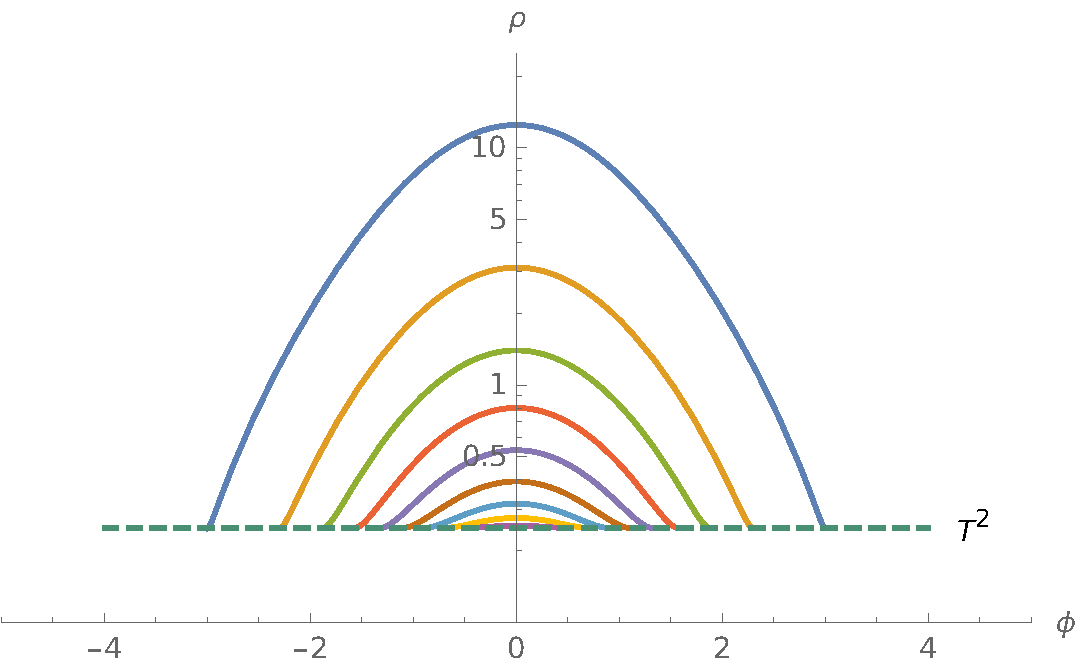
\includegraphics[width=.6\linewidth]{img/modFlowCutoff2BTZ.pdf}
%	\hspace{2em}
%	\vspace{-2ex}
	\caption[Integral surface of the modular flow when mapped to the planar BTZ coordinates]{%
		Integral surface of the modular flow when mapped to the planar BTZ coordinates. Note that the $\rho$ axis is logarithmic. 
		
		The flow starts from $t = 0,\ z = z_c$, and here we've chosen $\frac{L_\infty}{2} = 1$ while $z_c = 0.1,\,0.2,\,\cdots,\,0.9$. 
		Also we've taken $T_u = T_v = T = \frac{1}{2}$ as discussed before, and the horizon is at $\rho = T_u T_v = T^2$. 
	}
	\end{figure}
\subsection{The cutoff field theory perspective}
	From the field theory's perspective, the above calculations seem to suggest that the modular flow \underline{for an $L$-sized interval in the cutoff theory} is given by the modular flow \underline{of a CFT for an $L_\infty$ interval}; we denote this modular flow by $\xi = \xi(L_\infty)$. 
	
	One natural question is that whether this observation holds for a generic $T\bar{T}$ deformation, e.g.~the single-trace deformation of the opposite sign, which is dual to the TsT black string solution in the bulk, described by \textcite{Apolo:2019zai}. This will be explored in the later sections. The idea is:
	
	\begin{enumerate}
	\item There is a flow $f(\mu)$ from the undeformed $\mrm{AdS}/\mrm{CFT}$ to the deformed geometry, parametrized by $\mu$, that maps $L_\mrm{CFT}\mapsto L$. 
	In the cutoff picture, $f(\mu)$ moves the boundary into the bulk, and we have $L_\mrm{CFT} = L_\infty\mapsto L$. 
	
	Note that $f(\mu)$ is generally \textit{not} a diffeomorphism, otherwise the geometries will be equivalent; therefore, the action of $f(\mu)$ on quantities e.g.~the metric needs to be specified, and cannot be na\"ively induced from the map of coordinates. 
	
	\item The modular flow in the deformed theory is the ``push-forward'' of the CFT modular flow, namely $\xi_\mrm{CFT} \mapsto \xi = f^* \circ \xi_\mrm{CFT}$. However, such ``push-forward'' remains ambiguous, since $f(\mu)$ is \textit{not} a diffeomorphism, and we need an explicit prescription of this procedure.
	
	\item We then compute the entropy w.r.t.~the push-forward modular flow $\xi$, which is then reduced to the area of an RT surface in the deformed geometry. 
	
	\sidenote{The end result \textit{might} simply be a flow of the RT surface, induced by the flow $f(\mu)$ of the coordinates. Its area, on the other hand, depends on the flow of the metric.}
	\end{enumerate}
	This program echoes the idea advocated by \textcite{Guica:2019nzm}. 
\section{Entropy as Noether Charge}
	
	Ref: \textcite{Wald:1993nt,Iyer:1994ys,Iyer:1995kg}.
	
	Ref: \textcite{Lewkowycz:2013nqa}, \\
	\hspace*{4em} and \textcite{Faulkner:2013ana}.
	
	Gravitational entropy is the Noether charge $Q_\xi$ associated with some horizon generator $\xi$. In the case of entanglement entropy between a simple interval and its complement, we've found its corresponding modular flow in the bulk, which is precisely the horizon generator of the Rindler patch. We then aim to compute the charge variation using the covariant formula:
	\begin{equation}
		\var{Q}_{\xi} [\var{g}, g]
		= \int_{\pd\Sigma}
			\chi_\xi
		= \frac{1}{16 \pi G}
			\int_{\pd\Sigma}
			\sqrt{|g|} \dd{x}^{\alpha}
				\varepsilon_{\alpha\mu\nu}\,
				k_\xi^{\mu\nu} [\var{g}, g]
	\end{equation}
	\begin{equation}
	\begin{aligned}
		k_\xi^{\mu\nu}[\var g, g]
		= \frac{1}{2} \Big \{
		& \xi^{\nu}\nabla^{\mu} \var g^{\alpha}{}_{\alpha}
		- \xi^{\nu} \nabla_{\alpha} \var g^{\alpha\mu}
		+ \xi_{\alpha} \nabla^{\nu} \var g^{\alpha\mu}  \\
		&+ \frac{1}{2} \var g^{\alpha}{}_{\alpha} \nabla^{\nu} \xi^{\mu}
		- \frac{1}{2} \var g^{\nu\alpha} \nabla_{\alpha}\xi^{\mu}
		+ \frac{1}{2} \var g^{\nu\alpha} \nabla^{\mu} \xi_{\alpha} \\
		&- (\mu \leftrightarrow \nu) \Big \}
	\end{aligned}
	\label{kdef}
	\end{equation}
	However, to compute $\var{Q}$ we need to consider a particular metric variation $\var{g}_{\mu\nu}$ in the phase space of solutions. There is no free parameter in Poincar\'e $\mrm{AdS}_3$, unless we turn on temperature; this leads to the BTZ geometry. 
\subsection{Case study: BTZ}
	We thus have to repeat the calculations above to get the geodesic $\gamma$ and modular generators $\xi^\mu$ in the new BTZ backgrounds. However, it is convenient to remember that all BTZ black holes are locally equivalent to the pure $\mrm{AdS}_3$; we can then map Poincar\'e $(u,v,z)$ to BTZ Schwarzschild $(t,r,\phi)$ by \cite{Hubeny:2007xt}:
	\begin{equation}
		u,v = \sqrt{\frac{r^2 - r_+^2}{r^2 - r_-^2}}\,
			e^{(\phi\pm t)\,2T_{u,v}},
	\quad
		z = \sqrt{\frac{r_+^2 - r_-^2}{r^2 - r_-^2}}\,
			e^{\phi r_+ + t r_-},
	\end{equation}
	\begin{gather}
		r_\pm = T_u \pm T_v,
	\quad
		8GM = r_+^2 + r_-^2
		= 2\,(T_u^2 + T_v^2),
	\quad
		4GJ = r_+ r_-
		= T_u^2 - T_v^2,
	\end{gather}
	\begin{equation}
		\dd{s}^2
		= \frac{r^2 \dd{r}^2}{
				(r^2 - r_+^2)
				(r^2 - r_-^2)
			}
			+ T_u^2 \dd{u}^2
			+ T_v^2 \dd{v}^2
			+ (r^2 - T_u^2 - T_v^2) \dd{u} \dd{v}
	\end{equation}
	$\gamma$ and $\xi^\mu$ in BTZ coordinates both follow from this map. 
	
	What's the difference between this map and \eqref{eq:poincare2btz}? First, the coordinates are different: in \eqref{eq:poincare2btz} we have $(u,v,\rho)$ and here we have Schwarzschild $(t,r,\phi)$; but that's not essential. What's crucial is that here, we map \textbf{the \textsl{whole} of Poincar\'e into BTZ with a \textsl{compact} $\phi$ circle}, while before in \eqref{eq:poincare2btz} we map a \textbf{$L_\infty$-sized wedge in Poincar\'e into BTZ with a \textsl{non-compact} $\phi$ line}. 
	
	We now restrict to $t_\pm = 0, \phi_- = -\phi_+$ and again set $T_u = T_v = T$ for convenience; in this case the RT surface is given by \textcite{Rangamani:2016dms} (section 6.1.2):
	\begin{equation}
		r(\phi) = \frac{2T\cosh TL}{
				\sqrt{\cosh^2 TL - \cosh^2 2T\phi}
			}
	\end{equation}
	The charge variation has a nice form under the above simplifications; in this case we have $
		\var{Q}_{\xi}
		= \int \dd{x^\mu} (\chi_\xi)_\mu
	$, where e.g.
	\begin{equation}
		(\chi_\xi)_\phi
		= \frac{\var{T} \coth LT}{2G}
			\pqty{
				1 - {\frac{r}{\sqrt{r^2 - 4T^2}}}
				\frac{\cosh 2T\phi}{\cosh TL}
			}
	\end{equation}
	
	By definition the $\int_\gamma$ integration goes along the RT surface; we should be careful in the calculations and include the contributions from the $(\chi_\xi)_r \dd{r}$ component. 
	Alternatively, using Stokes' theorem, it can be done at the asymptotic infinity $r\to\infty$ instead; in this case we need only the $\phi$ component. These two integration contours give the same result:
	\begin{equation}
		\var{Q}_\xi
		= \frac{\var{T}}{2G} \pqty{
				L \coth LT - \frac{1}{T}
			}
	\end{equation}
	With a final integration w.r.t.~$\var{T}$ in the phase phase, we recover the resulting charge, which agrees with the entanglement entropy in \cite{Rangamani:2016dms} up to an overall constant shift:
	\begin{equation}
		Q_\xi = \frac{1}{2G} \log \frac{\sinh LT}{T}
	\end{equation}
	
\subsubsection{With constant cutoff}
	Now we consider constant cutoff at $r = r_c$. Again we need to trade the $L_\infty$ above with the coordinate length of the interval $L$ at the cutoff $r_c$. The relation can be solved by looking at the geodesic equation, which is slightly non-trivial this time:
	\begin{equation}
		\frac{\cosh L_\infty T}{\cosh LT}
		= \frac{r_c}{\sqrt{r_c^2 - 4T^2}}
	\end{equation}
	\begin{equation}
		r(\phi) = \frac{2T\cosh TL}{
				\sqrt{\cosh^2 TL - \pqty\big{
					1 - \frac{4T^2}{r_c^2}
				}\cosh^2 2T\phi}
			}
	\end{equation}
	We then compute the charges like before, and we have:
	\begin{equation}
		\var{Q}_\xi
		= \frac{\var{T}}{2G} \pqty{
				L \coth LT - \frac{1}{T}
			}
			\frac{1}{\sqrt{
				1 + \frac{4T^2}{r_c^2 \sinh^2 LT}
			}}
	\end{equation}
	
	We haven't found a nice way to compute this integral directly, but we note that the magical square root factor appears again in the $T\to 0$ limit:
	\begin{equation}
		T\to 0,
	\quad
		\sqrt{
			1 + \frac{4T^2}{r_c^2 \sinh^2 LT}
		}
		\to \sqrt{
			1 + \frac{4}{r_c^2 L^2}
		}
		\to \sqrt{
			1 + \frac{4z_c^2}{L^2}
		}
	\end{equation}
	This inspire us to take $L\pdd{L}$ first, and then compute the $\int \var{T}$; this is, surprisingly, doable, and reproduces the $C(L)$ function in \textcite{Lewkowycz:2019xse} in the $T \to 0$ limit:
	\begin{equation}
		L \pdv{L}\,Q_\xi
		= \frac{1}{2G}
			\frac{LT \coth LT}{\sqrt{
				1 + \frac{4T^2}{r_c^2 \sinh^2 LT}
			}},
	\quad\textsl{up to const.}
	\end{equation}
	
	Note that we have \textit{not} been very careful about the possible $L,T$ dependent integration constants. If we then do the $L$ integration from the above $L \pdv{L}\,Q_\xi$, we then find the charge up to some $L,T$ dependent integration constants:
	\begin{equation}
	\begin{aligned}
		Q_\xi
		&= \frac{1}{2G} \mop{arctanh}
			\frac{1}{\sqrt{
				1 + \frac{4T^2}{r_c^2 \sinh^2 LT}
			}}
		= \frac{1}{2G} \log
			\frac{
				\sqrt{
					1 + \frac{4T^2}{r_c^2 \sinh^2 LT}
				} + 1
			}{
				\sqrt{
					1 + \frac{4T^2}{r_c^2 \sinh^2 LT}
				} - 1
			},
	\quad\textsl{up to const.} \\
		&= \frac{1}{2G} \mop{arcsinh}
			\frac{r_c \sinh LT}{2T}
	\end{aligned}
	\end{equation}
	Although we haven't been careful about integration constants, this result happens to agree with the entropy in \cite{Lewkowycz:2019xse}. 
\section{Entanglement in the TsT Background}
	We are interested in the holographic entanglement entropy of the single-trace $T\bar{T}$ deformed theory, and we are considering the case where the deformation parameter carries a sign different from the cutoff picture. The setup is described by e.g.~\textcite{Apolo:2019zai,Chakraborty:2018kpr}. 
	
	Namely, we are considering a flow towards UV, instead of the flow towards IR studied by e.g.~\cite{McGough:2016lol,Lewkowycz:2019xse}. 
	The field theory side calculation of entanglement entropy \cite{Donnelly:2018bef,Lewkowycz:2019xse} seems to survive through the sign flip; when dualed to the bulk it suggests that:
	\begin{equation}
		S = \frac{1}{2G} \mop{arccosh}
			\frac{L}{L_0},
	\quad
		C(L) = L \pdv{L}\,S
		= \frac{1}{2G} \frac{1}{
				\sqrt{1 - (\frac{L_0}{L})^2}
			}
	\label{eq:tst_ft_ee}
	\end{equation}
	There is a length scale $L_0$ here which is the minimal length of the entanglement interval; for $L < L_0$ the entropy becomes complex, thus unphysical. This can be interpreted as a UV length scale arised from the deformation. In terms of the worldsheet deformation parameter $\lambda$ and w.r.t.~to the TsT metric given in \cite{Apolo:2019zai}, we have:
	\begin{equation}
		L_0 = \sqrt{8\lambda}
	\end{equation}
	
	Although we've expressed everything in terms of the bulk parameters and the worldsheet deformation parameter $\lambda$, we'd like to emphasize that the above results comes from purely field theoretical calculations, and they are mapped to the bulk using the holographic dictionary. Our goal is to reproduce them as gravitational entropy, from bulk calculations. 
\subsection{Case study: Ramond vacuum $T_u = T_v = 0$}
	For simplicity, we first look at the \textsl{Ramond vacuum}, i.e.~the TsT background with $T_u = T_v = 0$. In this case the string frame metric and dilaton is given by:
	\begin{equation}
		\dd{s}^2
		= \frac{\dd{z}^2}{z^2}
			+ \frac{\dd{u}\dd{v}}{z^2 + 2\lambda},
	\quad
		e^{2\Phi}
		= \frac{k}{p}
			\frac{z^2}{z^2 + 2\lambda}\,
			e^{-2\phi_0},
		\label{eq:staticMetricPoincare}
	\end{equation}
	To avoid confusion with the dilaton, we denote the angular direction with the curvy $\varphi = \frac{u + v}{2}$. 
	This is derived from (3.13) of \cite{Apolo:2019zai}, with $r = \frac{1}{z^2}$; we've set the AdS radius $\ell_{\mrm{AdS}} = 1$ for now and neglected the $B$ field. For more simplifications, we further set:
	\begin{equation}
		p = k = 1
	\end{equation}
\subsubsection{The usual RT surface}
	The Einstein frame metric $G_{\mu\nu}$ is related to the string frame metric $g_{\mu\nu}$ by:
	\begin{equation}
		G_{\mu\nu} = e^{-4\Phi} g_{\mu\nu}
	\end{equation}
	Now consider a spacelike geodesic in Einstein frame within the time slice $t = 0$; we can nicely parametrize it  with its peak $z_0$ at $\varphi = 0$. The $\pdd{\varphi}$ symmetry implies that along the geodesic $\gamma$,
	\begin{equation}
		\pqty{\dv{z}{\varphi}}_{\!\gamma}^{\!2}
		= \frac{z_0^2}{z^2}
				\frac{z_0^2}{z_0^2 + 2\lambda}
			- \frac{z^2}{z^2 + 2\lambda}
	\end{equation}
	
	The coordinate length $L_\mrm{RT}$ at the boundary is given by:
	\begin{equation}
	\begin{aligned}
	  L_\mrm{RT} = L_\mrm{RT}(z_0;\lambda)
	  &= \int \dd{\varphi}
	  = 2\int_0^{z_0}
	      \abs{\dv{\varphi}{z}}
	      \dd{z} \\
	  &= 2\int_0^{z_0}
	      \frac{1}{\sqrt{
	          \frac{z_0^2}{z^2}
	          \frac{z_0^2}{z_0^2 + 2\lambda}
	          - \frac{z^2}{z^2 + 2\lambda}
	      }}
	      \dd{z}
	\end{aligned}
	\label{eq:length_function}
	\end{equation}
%	
%\pagebreak\noindent
	Note that:
	\begin{itemize}
	\item $\lambda\to 0$, \textsl{or} $z_0\to \infty$, we have $L_\mrm{RT}(z_0;\lambda) \to 2z_0$, i.e.~we recover the AdS result: in this case the geodesic $\gamma$ is a semi-circle with radius $z_0$.
	
	\item $z_0\to 0,\,
		L_\mrm{RT}(z_0;\lambda) \to \sqrt{\frac{\pi^2}{2} \lambda}
	$, we see that $L_\mrm{RT}$ seems to be bounded from below by:
	\begin{equation}
		L_{\mrm{RT},0} (\lambda)
		= \sqrt{\frac{\pi^2}{2} \lambda}
	\end{equation}
	This feature is very similar to the lower bound $L_0$ of entanglement length, but they do \textit{not} agree; in fact,
	\begin{equation}
		L_{\mrm{RT},0} / L_0 = \pi / 4
	\end{equation}
	\end{itemize}
	
	The entanglement entropy, as proposed by RT, is given by:
	\begin{equation}
	\begin{aligned}
	  S_\mrm{RT}
	  &= \frac{1}{4G} \int_\gamma
	    \frac{z^2 + 2\lambda}{z^2}
	    \sqrt{
	        \frac{\dd{z}^2}{z^2}
	        + \frac{\dd{\varphi}^2}{z^2 + 2\lambda}
	    } \\
	  &= \frac{1}{2G} \int_0^{z_0} \dd{z}
	    \frac{z^2 + 2\lambda}{z^2}
	      \sqrt{
	          \frac{1}{z^2}
	          + \frac{1}{z^2 + 2\lambda}
	          \Big/
	          \pqty{\dv{z}{\varphi}}^{\!\!2}
	      } \\
	  &= \frac{1}{2G} \int_0^{z_0} \dd{z}
	    \frac{z^2 + 2\lambda}{z^2}
	      \sqrt{
	          \frac{1}{z^2}
	          + \frac{1}{z^2 + 2\lambda}
	          \Big/
	          \pqty{
					\frac{z_0^2}{z^2}
					\frac{z_0^2}{z_0^2 + 2\lambda}
					- \frac{z^2}{z^2 + 2\lambda}
	          }
	      }
	\end{aligned}
	\label{eq:RT_integral}
	\end{equation}
	We don't have an explicit analytic result for the above integral\footnote{
		Note that there are some analytic expressions given by \cite{Asrat:2019end}, but we haven't confirmed their results. 
		We can map \cite{Asrat:2019end} to our convention by matching the aysmptotic behavior of $L_\mrm{RT}$; namely, we have $z_0 \to \infty$, $L_\mrm{RT}(z_0;\lambda)\to 2z_0$, while $z_0 \to 0$, $L_\mrm{RT}(z_0;\lambda)\to \sqrt{\frac{\pi^2}{2} \lambda}$. It seems that for (3.17) and (4.3) in \cite{Asrat:2019end}, we have $
			\alpha \mapsto \frac{\lambda/2}{z^2}
		$. With this the length $L_\mrm{RT}$ given by \cite{Asrat:2019end} as a function of $z$ is \textit{not} monotonic, which sounds suspicious and does not agree with numerical results. \label{foot:asrat_matching}
	},
	but numerical calculations suggest that it does not agree with \eqref{eq:tst_ft_ee}. \sidenote{However, its qualitative behavior is quite close to \eqref{eq:tst_ft_ee}, and it fits \eqref{eq:tst_ft_ee} nicely as $L\to \infty$. }
	
\pagebreak[3]
	
	As is inspired by the cutoff picture, we would like to tweak the holographic entropy such that it matches with \eqref{eq:tst_ft_ee}. 
	We start with the following observations: 
	\begin{itemize}
	\item If we denote $L_{\mrm{CFT}} = 2z_0$, and instead of using \eqref{eq:length_function}, we use:
	\begin{equation}
		L' = 2\sqrt{z_0^2 + 2\lambda},
	\quad\text{i.e.}\quad
		\pqty{\frac{L'}{2}}^{\!\!2}
		= \pqty{\frac{L_\mrm{CFT}}{2}}^{\!\!2} + 2\lambda,
	\end{equation}
	Which mimic the relation \eqref{eq:length_relations}, then the $C(L)$ from the field theory calculations can be re-written as:
	\begin{equation}
		C(L')
		= \frac{1}{\sqrt{1 - (\frac{L_0}{L'})^2}}
		= \frac{L'}{L_{\mrm{CFT}}},
	\quad L_0 = \sqrt{8\lambda}
	\end{equation}
	Where the relation $C(L') = \frac{L'}{L_{\mrm{CFT}}}$ is completely analogous to the double-trace situation; in that case we have $L_\mrm{CFT} = L_\infty$. 
	
	\pagebreak[3]
	
	\item Maybe one can ``engineer'' a suitable curve $\gamma'$ which has peak $z_0$ and boundary length $
		L' = 2\sqrt{z_0^2 + 2\lambda}
	$; we can require that it reproduces the desired entanglement entropy \eqref{eq:tst_ft_ee}:
	\begin{equation}
		\frac{1}{2G} \mop{arccosh}
			\frac{
				\sqrt{z_0^2 + 2\lambda}
			}{\sqrt{2\lambda}}
	  = \frac{1}{2G} \int_0^{z_0} \dd{z}
	    \frac{z^2 + 2\lambda}{z^2}
	      \sqrt{
	          \frac{1}{z^2}
	          + \frac{1}{z^2 + 2\lambda}
	          \pqty{\dv{\varphi}{z}}^{\!\!2}
	      } 
	\end{equation}
	This is a integral equation for $\dv{\varphi}{z} \equiv F$. The above equation can be greatly simplified by:
	\begin{equation}
		z = \sqrt{2\lambda} \sinh y,
	\quad
		F(y;y_0,\lambda)
		= \abs{\dv{\varphi}{z}},
	\end{equation}
	\begin{empheq}{equation}
		y_0
		= \int_0^{y_0} \dd{y}
			\coth^2 y\,\sqrt{
				\coth^2 y
				+ F^2(y;y_0,\lambda)
			}
	\end{empheq}
	
	$z_0$ or $y_0$ labels the peak of $\gamma$, thus we have:
	\begin{empheq}{equation}
		F(y\to y_0;y_0,\lambda) \to \infty
	\end{empheq}
	Also the boundary length should be:
	\begin{gather}
	  L' = 2\sqrt{z_0^2 + 2\lambda}
	  = 2\int_0^{z_0}
	      \abs{\dv{\varphi}{z}}
	      \dd{z},
	\end{gather}
	\begin{empheq}{equation}
		\cosh y_0
		= \int_0^{y_0}
			F(y;y_0,\lambda) \cosh y \dd{y}
	\end{empheq}
	
	In principle one might be able to find some candidate $F = F(y;y_0,\lambda)$ from the boxed equations. This corresponds to candidate curve $\gamma'$ that reproduces the desired entropy. 
	
	\item There is a $B$-field in the TsT background; however, as is argued in \texttt{areaTTbar.pdf}, it should not contribute to the on-shell action. However, one might be able to promote the original $\gamma_\mrm{RT}$ to a tube surrounding $\gamma_\mrm{RT}$, and treat it as a string worldsheet, where the $B$-field couples nicely in the worldsheet action. 
	
	There are two ways going forward: one is to compute the string EoMs which is related to the \textit{string frame} geodesic; this is done in \texttt{notesEETTbar.pdf} and to be discussed in the next section. 
	
	\sidenote{Another way is to come up with a procedure that reduces the string action to a particle action close to $S_{\mrm{RT}}$, but with $B$-field corrections. One can also construct a new connection with $H = \dd{B}$ and solve the geodesic with this new connection\footnote{
		Thank Yuan Zhong for this great idea. Also he helped a lot with simplying the integral equations. 
	}. }
	
	\item With quite a bit of numeric experimentations, we find that:
	\begin{equation}
		L_\mrm{CFT}\,\pdv{L_\mrm{CFT}}\,S_\mrm{RT}
		= z_0\,\pdv{z_0}\,S_\mrm{RT}
		\sim \frac{1}{2G}
	\label{eq:RT_entropy_derivative}
	\end{equation}
	In fact the result seems to be $\lambda$ independent; but we know that:
	\begin{equation}
		S_{\lambda = 0}
		= \frac{1}{2G}
			\log \frac{L_\mrm{CFT}}{\epsilon}
		= \frac{1}{2G}
			\log \frac{2z_0}{\epsilon}
	\end{equation}
	Namely $
		z_0\,\pdv{z_0}\,S_{\lambda = 0}
		= \frac{1}{2G}
	$ exactly. Combined with the numerical results, this hints at the fact that \eqref{eq:RT_entropy_derivative} holds exactly with no $\lambda$ dependence. 
	
	However, if we use the analytic result of \cite{Asrat:2019end} (see footnote \ref{foot:asrat_matching}), then this is \textit{not} correct! But one should check that result first to see if it's valid first.
	\sidenote{Also,} if we take the $z_0$ derivative before integrating in \eqref{eq:RT_integral}, we can show that indeed we have, approximately, $
		z_0\,\pdv{z_0}\,S_\mrm{RT}
		\approx \frac{1}{2G}
	$, but the result is \sidenote{\textit{not} exactly constant and \textit{not} $\lambda$ independent;} see \texttt{zDzNonConstant.nb}. 
	
\pagebreak[3]
	
	If we proceed anyways with $
		z_0\,\pdv{z_0}\,S_\mrm{RT}
		\approx \frac{1}{2G}
	$, then we have:
	\begin{equation}
		L' \pdv{S_\mrm{RT}}{L'}
		= L_\mrm{CFT} \pdv{S_\mrm{RT}}{L_\mrm{CFT}}
			\pdv{L_\mrm{CFT}}{L'}
			\frac{L'}{L_\mrm{CFT}}
		\approx \frac{1}{2G}
			\pqty{\frac{L'}{L_\mrm{CFT}}}^{\!\!2}
		= C(L')^2
	\end{equation}
	We find that \textit{numerically}, this does hold very well. Unfortunately this is not what we expected. How should we interpret this?
	\end{itemize}
	
	\begin{figure}[!ht]
	\centering
	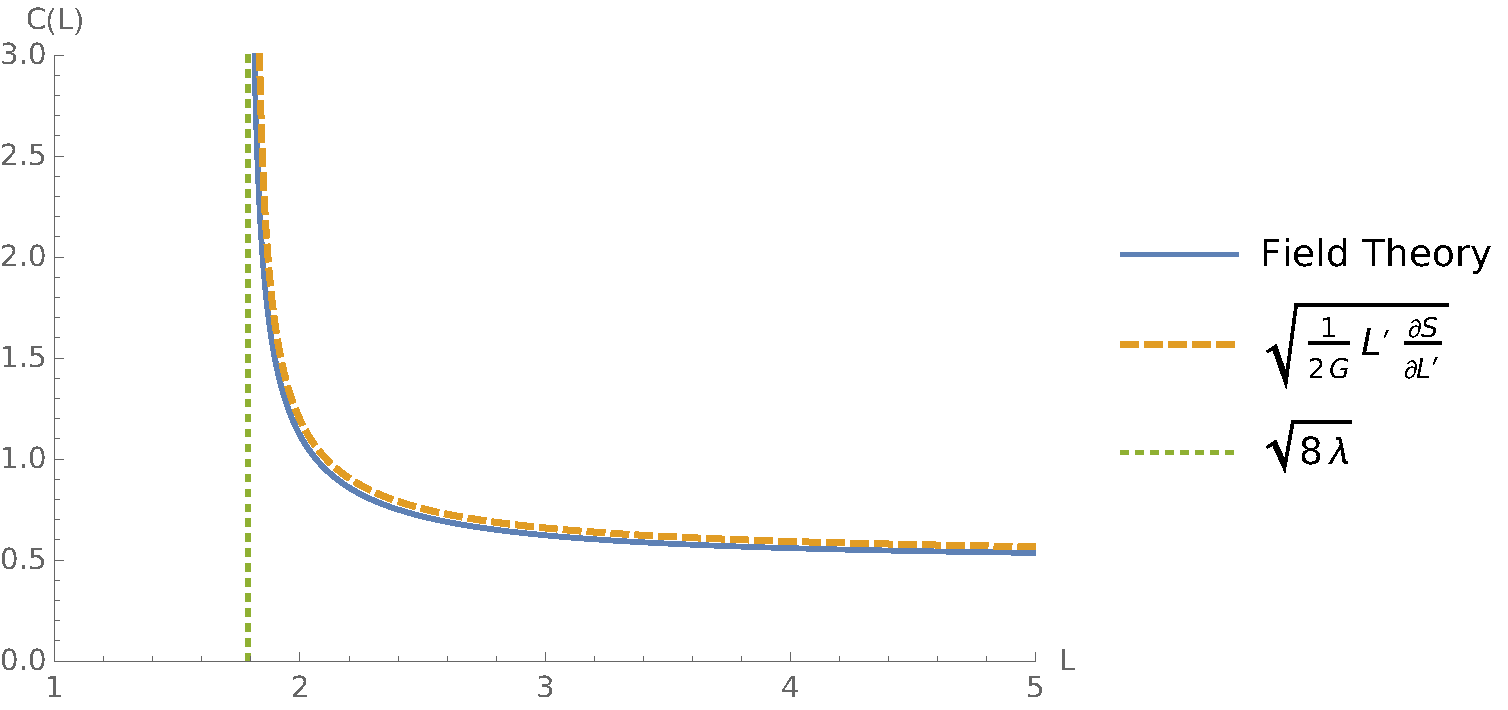
\includegraphics[width=.7\linewidth]{img/cFunctionGame.pdf}
%	\hspace{2em}
%	\vspace{-2ex}
	\caption[Numerical construction of the $C(L)$ function]{%
		Numerical construction of the $C(L)$ function from $S_\mrm{RT}$ by considering $
			\sqrt{
				\frac{1}{2G}
				L' \pdv{S}{L'}
			}
		$. What's happening? I have no idea. \sidenote{Update: it seems that this only holds approximately, perhaps it's simply a numerical coincidence. }
	}
	\end{figure}
\subsubsection{The TsT deformed geodesic}
	If we take the usual geodesic (semi-circle) in the undeformed background, and consider a TsT transformation, we get the TsT deformed geodesic $\gamma_\mrm{TsT}$. This also coincides with the \textit{string frame} geodesic, which minimizes the string frame length without the dilaton factor, instead of the Einstein frame length. See \texttt{notesEETTbar.pdf} for a description of this process. 
	
	However, the on-shell action should still be the Einstein frame length; fortunately, this time the result is nice and clean:
	\begin{equation}
		S_E[\gamma_\mrm{TsT}(z0;\epsilon)]
		= \frac{1}{2}
			\frac{\sqrt{z_0^2 + 2\lambda}}{z_0}
			\pqty{
				\frac{\lambda}{\epsilon^2}
				\frac{\sqrt{z_0^2 - \epsilon^2}}{z_0}
				+ \frac{z_0^2 + \lambda}{z_0^2}
				\mop{arctanh}
					\frac{\sqrt{z_0^2 - \epsilon^2}}{z_0}
			}
	\end{equation}
	Unfortunately, the result is highly divergent: $\sim \frac{1}{\epsilon^2}$, even worse than the $\log \frac{1}{\epsilon}$ divergence of a CFT. 
	\sidenote{It might be possible to "renormalize" out the $\sim \frac{1}{\epsilon^2}$ divergence} which might also help us recover a more reasonable on-shell action.
	
\vspace{1.2\baselineskip}
\pagebreak[4]
\raggedright
\printbibliography[%
%	title = {参考文献} %
	,heading = bibintoc
]
\end{document}
